
\begin{frame}
    \frametitle{Transient period: Decision chart}
    \begin{equation*}
      T_a = \frac{\epsilon}{2}\left(\frac{1}{a^+}- \frac{1}{a^-}\right) + \frac{u+w}{\epsilon}(T^f_{\sigma_x}-T^{0}_{\sigma_x})
    \end{equation*}
  
    \begin{columns}
      \column{0.5\textwidth}
      \uncover<-1>{  
      \textbf{Anticipation Time}
        \begin{figure}
          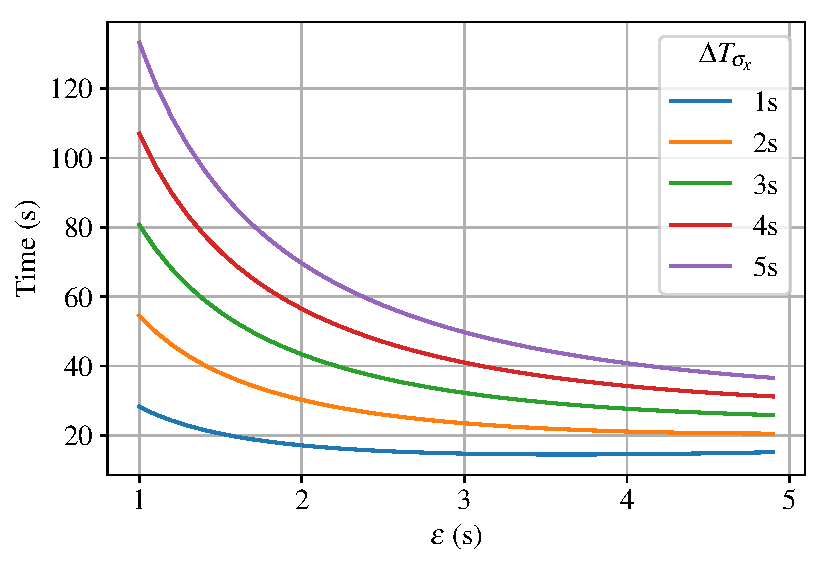
\includegraphics[width=0.9\linewidth]{fig_11a_anticipation_time.pdf}\hspace*{1cm}
        \end{figure}
      }
      \column{0.5\textwidth}
      \uncover<-1>{
      \textbf{Speed drop}
        \begin{figure}
          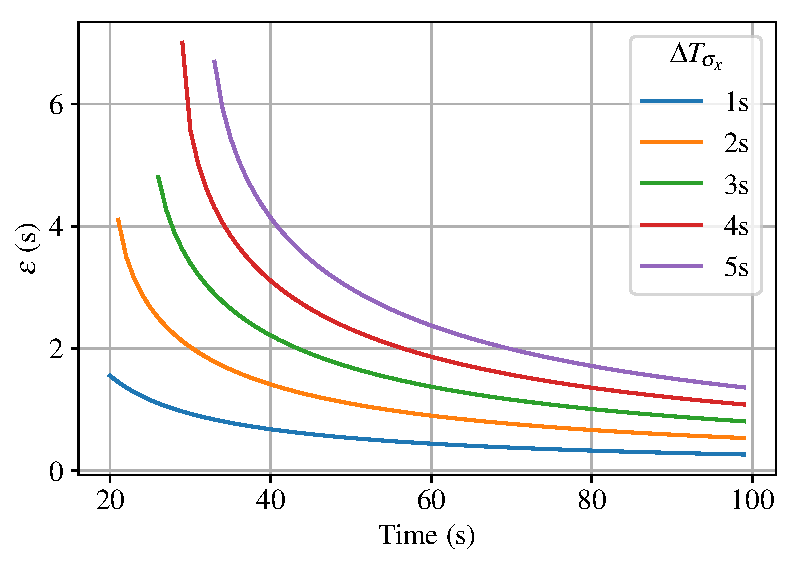
\includegraphics[width=0.9\linewidth]{fig_11b_anticipation_time.pdf}\hspace*{1cm}
        \end{figure}
      }
    \end{columns}
  \end{frame}